\lstset{style=bash}

\section{Organisation of the repository}

	\begin{minipage}{0.65\linewidth}
		For the organisation of the repository, we created several directories (Figure \ref{tree}):
		\begin{enumerate}[label=\textbullet]
			\item \textbf{src :} In this directory there is all the source code of the project. We have a first \textit{Python} subdirectory which contains the Python codes for the data assimilation and parareal parts : these files were created during the M1 project. Then, we have a second subdirectory \textit{cpp} which contains the C++ codes of the same two parts.
			\item \textbf{examples :} Here there are examples of how to use the Python and C++ codes.
			\item \textbf{tests :} In this directory there are Python and C++ tests of the code. For Python tests we have used the pytest tool and for C++ we have used ctest (see Appendix \ref{compile}).
			\item \textbf{docs :} This directory gathers all the files that are used to generate the documentation of the project (see Appendix \ref{doc}). The \textit{sphinx} and \textit{doxygen} directories enable respectively to document the Python code and the C++ code (thanks to the Sphinx~\cite{sphinx_doc} and Doxygen~\cite{doxygen_doc} tools). The \textit{antora} directory contains some explanations of the project which are accessible online (the Antora~\cite{antora_doc} tool was used). For example it explains : the differential equations treated in this project, the data assimilation methods, the parareal method... The documentations generated by the previous tools are available directly in the GitHub repository via a Continuous Integration (CI), framework that has been set up (see Appendix \ref{ci}).
			The directories \textit{gantt}, \textit{meeting}, \textit{presentation} and \textit{report} contain all the \LaTeX ~files and images used for the presentations and reports requested in the context of the internship.
			\item \textbf{cmake/build :} The directory \textit{cmake} contains cmake configuration files which are used for the compilation of the C++ project (see Appendix \ref{compile}). The directory \textit{build} contains all the files generated by the compilation of the C++ code.
		\end{enumerate}
	\end{minipage} \qquad
	\begin{minipage}{0.33\linewidth}
		\begin{figure}[H]
			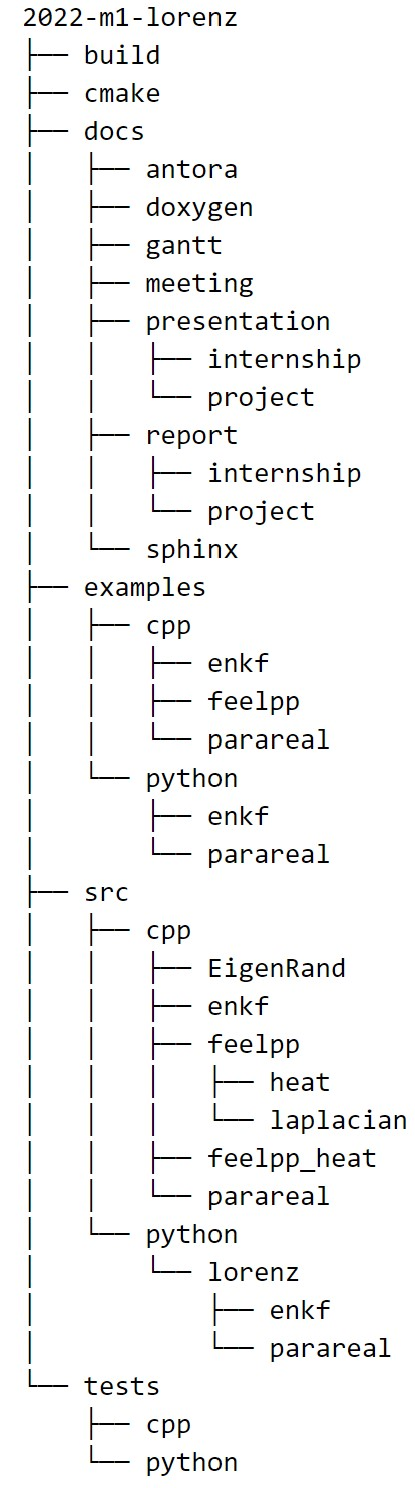
\includegraphics[width=\textwidth]{"images/appendix/tree.jpg"}
			\caption{Repository tree}
			\label{tree}
		\end{figure}
		%\lstinputlisting[language={},inputencoding=utf8]{tree.txt}
	\end{minipage}

\newpage

\section{Compile and test}
\label{compile}

	As explained in the previous section, the project includes both C++ and Python code. Let's see how to use these source codes :
	\begin{enumerate}[label=\textbullet]
		\item \textbf{Python :} \\
		Here all methods are grouped in a module called \textit{lorenz}. To execute the examples, we first need to add the path to the source code in the PYTHONPATH variable using the following command at the root of the project :
\begin{lstlisting}
		export PYTHONPATH=$PWD/src/python
\end{lstlisting}
		\fbox{ENKF ?} \\
		To run the examples for the parareal method with 2 processes, go to "examples/python/parareal" and then execute :
\begin{lstlisting}
		mkdir data_parareal
		mpirun -n 2 python3 examples_parareal.py [0,1,2]
\end{lstlisting}
		To run the tests we use the Pytest tool. To do this, go to "tests/python" and run the following command :
\begin{lstlisting}
		pytest
\end{lstlisting}
		\item \textbf{C++ :} \\
		For the C++ code, we decided to write a CMake\footnote[1]{Minimum version required : 3.21} file with presets~\cite{cmake_preset}.  A recurrent problem of CMake users is to share settings with other people for common ways of configuring a project. A solution to this is to create a "CMakePresets.json" file at the root of the project allowing to define different compilation modes. \\
		We defined 3 presets : \textit{default} is the default compilation mode, \textit{dbg} the mode to debug the code and \textit{doc} to generate the documentation (see Appendix \ref{doc}). \\
		These are the commands to configure and build in default mode :
\begin{lstlisting}
		cmake --preset default
		cmake --build --preset default
\end{lstlisting}
		The executables generated by the last command will then be stored in the "build/default/bin" directory. There you will find :
		\begin{itemize}[label=-]
			\item \textbf{enkf.e : } \fbox{ENKF ?}
			\item \textbf{parareal.e : } To run in parallel with 4 processes :
\begin{lstlisting}
		mpirun -n 4 ./build/default/bin/parareal.e
\end{lstlisting}
			This applies the parareal method to the Lorenz system with parameters defined in the code and displays the number of iterations of the method as well as the execution time. 
			\item \textbf{laplacian.e : } To run in sequential:
\begin{lstlisting}
		./build/default/bin/laplacian.e 
				--config-file <cfg_filename>
\end{lstlisting}
			To run in parallel with 4 processes:
\begin{lstlisting}
		mpirun -n 4 ./build/default/bin/laplacian.e 
				--config-file <cfg_filename>
\end{lstlisting}
			This allows to solve the Laplace equation on a given geometry via the finite element method by using Feel++~\cite{feelpp_laplacian}.
			\item \textbf{heat.e : } \\
			This solves in parallel the heat equation on a given geometry with the parareal method by using Feel++. \\
			We will place ourselves in the following test case :
			\begin{enumerate}[label=\ding{213}]
				\item The spatial domain is partitioned into 2 sub-domains using the command :
\begin{lstlisting}
		feelpp_mesh_partitioner --dim=2 --part 2 
				--ifile <geo_filename> 
\end{lstlisting}
			\item We also partition the temporal domain into 2 sub-domains, which makes 2*2 processes for the fine integrator and 2 processes for the coarse integrator, so 6 processes in all. We can then run in parallel with 6 processes :
\begin{lstlisting}
		mpirun -np 6 ./build/default/bin/heat.e 
				--config-file <cfg_filename>
\end{lstlisting}		
		\end{enumerate}
		For more details see Section \ref{heat}.
		\end{itemize}
		For C++ tests, we use the Ctest tool in the following way:
\begin{lstlisting}
		ctest --preset default
\end{lstlisting}
	\end{enumerate}

\newpage

\section{Documentation}
\label{doc}

	To document the project, we have used different tools. As said before, all the files concerning the documentation are in the \textit{docs} directory. \\
	Before presenting these tools, it's important to note that we have set up a Continuous Integration routine in order to automatically generate this documentation when a push is made on GitHub (see Section \ref{ci}). \\
	Here is the link to the documentation : \url{https://master-csmi.github.io/2022-m1-lorenz/}. \\
	To document the project we used 3 tools:
	\begin{itemize}[label=-]
		\item \textbf{Sphinx\cite{sphinx_doc}} : To document the Python code. 
		\item \textbf{Doxygen\cite{doxygen_doc}} : To document C++ code.
		\item \textbf{Antora\cite{antora_doc}} : To explain some parts/methods of the project (and to be able to keep the documentation online).
	\end{itemize}
	We will now see how to generate the documentation locally using these 3 tools. For that, there are 2 methods : the first one is to generate "manually" the html files and the second one is to use the \textit{docs} preset of our CMake.
	\begin{enumerate}[label=\textbullet]
		\item \textbf{Manual generation :} 
		\begin{itemize}[label=-]
			\item \textbf{Antora :} Go to "docs/antora", then execute :
\begin{lstlisting}
		npm install
		npm run dev
		npm run serve
\end{lstlisting}
			Then click on the following link (in the "site-dev.yml" file) : \\ \url{http://127.0.0.1:8080/lorenz/1.0.0/index.html}. \\
			If we modify the documentation files, we just have to re-run the second line which will regenerate the documentation and then reload our browser window.
			\item \textbf{Sphinx :} Go to "docs/sphinx", then execute :
\begin{lstlisting}
		make html
		npm run sphinx
\end{lstlisting}
			\item \textbf{Doxygen :} Go to "docs/doxygen", then execute :
\begin{lstlisting}
		doxygen Doxyfile-dev.in
		npm run doxygen
\end{lstlisting}
		\end{itemize}
		\newpage
		\item \textbf{With CMake :} \\
		\danger This method is only available for Sphinx and Doxygen documentations. Indeed, CMake is configured so that Antora documentation is generated from the files uploaded online on Github. This configuration is due to CI (see Section \ref{ci}). This means that local modifications will not be taken into account with this method. \\ \; \\
		Here is how to use the CMake \textit{docs} preset to generate the Sphinx and Doxygen documentations (by placing at the root of the project) :
\begin{lstlisting}
		cmake --preset docs
		cmake --build --preset docs
\end{lstlisting}
		Then in the same way as before, execute one of the following commands at the root of the project :
\begin{lstlisting}
		npm run sphinx
\end{lstlisting}
		or
\begin{lstlisting}
		npm run doxygen
\end{lstlisting}
	\end{enumerate}

\newpage

\section{Github actions}
\label{ci}

	As said before we have set up a CI (Continuous Integration) using GitHub actions.
	We added a badge at the beginning of the readme of our project to see when the build passed and when the build failed. Here is what it looks like in both cases : \\
	\begin{minipage}{0.48\linewidth}
		\begin{figure}[H]
			\centering
			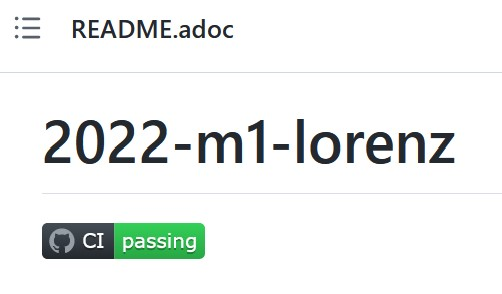
\includegraphics[width=0.45\textwidth]{"images/appendix/badge_ok.jpg"}
			\caption{Build passing}
			\label{badge_ok}
		\end{figure}
	\end{minipage}
	\begin{minipage}{0.48\linewidth}
		\begin{figure}[H]
			\centering
			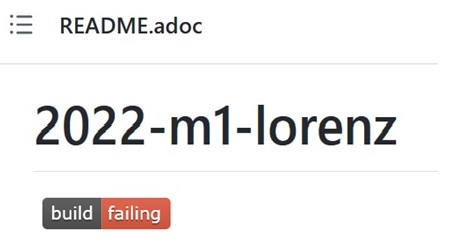
\includegraphics[width=0.5\textwidth]{"images/appendix/badge_not_ok.jpg"}
			\caption{Build failing}
			\label{badge_not_ok}
		\end{figure}
	\end{minipage} \\ \; \\
	For more details, in the action tab of the repository all the tasks of each commit are specified. Here is a preview of the CI for one commit :
	\begin{figure}[H]
		\centering
		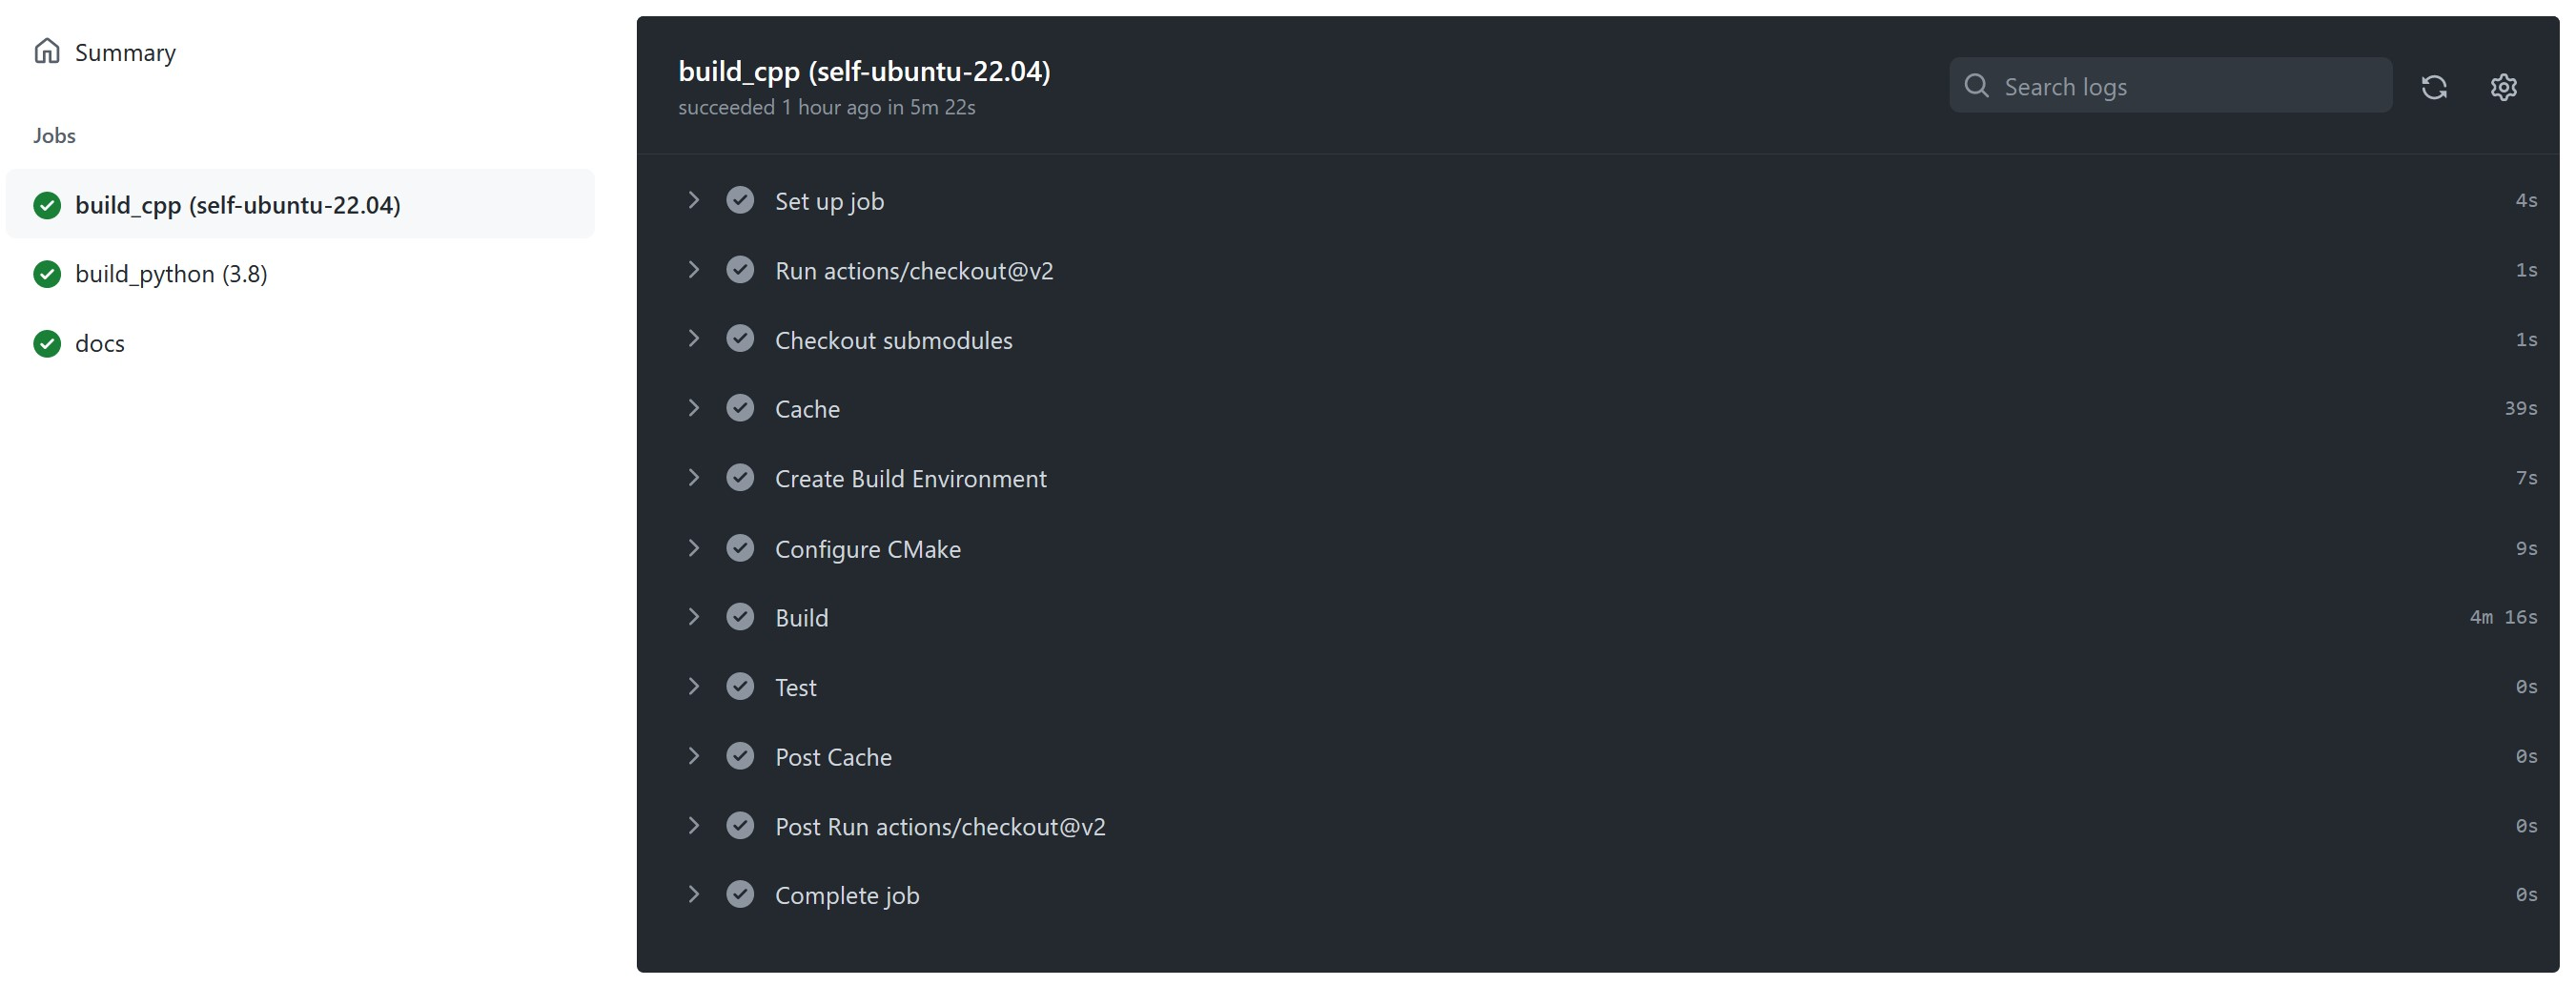
\includegraphics[width=0.65\textwidth]{"images/appendix/run_ci.jpg"}
		\caption{Tab actions in GitHub (for one commit example)}
		\label{run_ci}
	\end{figure}
	\noindent Here are the jobs realized as soon as we push in the main branch :
	\begin{enumerate}[label=\textbullet]
		\item Compile C++ code using CMake default preset, then use ctest to check if the tests pass.
		\item Test the Python code with pytest.
		\item Generate the documentation (Sphinx, Doxygen and Antora) using the docs preset of the CMake. Then, deploy the 3 documentations in the \textit{gh-pages} branch (in 3 respective directories: \textit{build\_sphinx}, \textit{build\_doxygen} and \textit{build\_antora)}. An html file has been created manually at the root of this branch in order to group the 3 documentations :
		\begin{figure}[H]
			\centering
			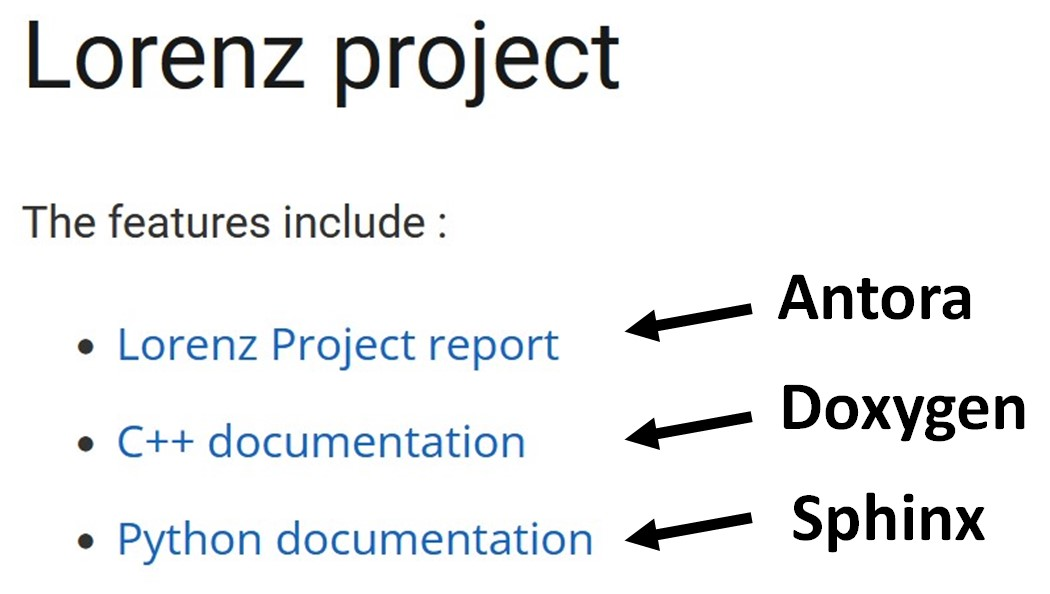
\includegraphics[width=0.25\textwidth]{"images/appendix/html_file.jpg"}
			\caption{Main page of the documentation}
			\label{html_file}
		\end{figure}
		For more details about the documentation see Section \ref{doc}.
	\end{enumerate}